% !TEX program = xelatex
\makeatletter\let\@expl@@@mark@update@singlecol@structures@@\relax\makeatother
\documentclass[a4paper,10pt]{article}

% -------------------- កញ្ចប់ពុម្ពអក្សរ និងភាសា --------------------
\usepackage{fontspec}
\usepackage{amsmath,amssymb}
\usepackage{unicode-math}
\usepackage{pifont}

% -------------------- ការកំណត់ទំព័រ (Page Setup — លំនាំ ls_plan.tex) --------------------
\usepackage[
  a4paper,
  left=0.95cm,
  right=0.95cm,
  top=0.85cm,
  bottom=0.92cm,
  footskip=0.52cm
]{geometry}

\usepackage{fancyhdr}
\usepackage{lastpage}
\usepackage{array}
\usepackage{longtable}
\usepackage{multirow}
\usepackage{colortbl}
\usepackage[table]{xcolor}
\usepackage{enumitem}
\usepackage{tikz}
\usetikzlibrary{calc,angles,quotes,arrows.meta,decorations.pathreplacing,patterns}
\usepackage[most]{tcolorbox}

% -------------------- ពុម្ពអក្សរផ្លូវការ (Cross-Platform \NGSFindFonts) --------------------
\providecommand{\NGSFindFonts}{%
  \IfFileExists{C:/Windows/Fonts/cambria.ttc}{%
    \def\NGSSysPath{C:/Windows/Fonts/}%
    \def\NGSUserPath{C:/Users/KIT/AppData/Local/Microsoft/Windows/Fonts/}%
  }{%
    \IfFileExists{./fonts/KhmerOSsiemreap.ttf}{\def\NGSSysPath{./fonts/}\def\NGSUserPath{./fonts/}}{%
    \IfFileExists{../fonts/KhmerOSsiemreap.ttf}{\def\NGSSysPath{../fonts/}\def\NGSUserPath{../fonts/}}{%
    \IfFileExists{../../fonts/KhmerOSsiemreap.ttf}{\def\NGSSysPath{../../fonts/}\def\NGSUserPath{../../fonts/}}{%
    \IfFileExists{../../../fonts/KhmerOSsiemreap.ttf}{\def\NGSSysPath{../../../fonts/}\def\NGSUserPath{../../../fonts/}}{%
    \IfFileExists{../../../../fonts/KhmerOSsiemreap.ttf}{\def\NGSSysPath{../../../../fonts/}\def\NGSUserPath{../../../../fonts/}}{%
    \IfFileExists{../../../../../fonts/KhmerOSsiemreap.ttf}{\def\NGSSysPath{../../../../../fonts/}\def\NGSUserPath{../../../../../fonts/}}{%
    \IfFileExists{../../../../../../fonts/KhmerOSsiemreap.ttf}{\def\NGSSysPath{../../../../../../fonts/}\def\NGSUserPath{../../../../../../fonts/}}{%
      \def\NGSSysPath{../../../../../../../fonts/}\def\NGSUserPath{../../../../../../../fonts/}%
    }}}}}}}%
  }%
}
\NGSFindFonts

\setmathfont[Path={\NGSSysPath}, FontIndex=1, Scale=1.02]{cambria.ttc}
\defaultfontfeatures{Ligatures=TeX}

\setmainfont[
  Path={\NGSUserPath}, Extension=.ttf, Script=Khmer,
  BoldFont={KhmerOSsiemreap}, BoldFeatures={FakeBold=1.8},
  ItalicFont={KhmerOSsiemreap}, ItalicFeatures={FakeSlant=0.25},
  BoldItalicFont={KhmerOSsiemreap}, BoldItalicFeatures={FakeBold=1.8, FakeSlant=0.25}
]{KhmerOSsiemreap}

\newfontfamily\muol[Path={\NGSUserPath}, Extension=.ttf, Script=Khmer]{KhmerOSmuollight}
\newfontfamily\TimesEn[Path={\NGSSysPath}, Extension=.ttf, BoldFont={timesbd}, ItalicFont={timesi}, BoldItalicFont={timesbi}]{times}
\newfontfamily\NagaBold[Path={\NGSUserPath}, Extension=.ttf]{AKbalthom Naga Bold}
\newfontfamily\CalibriFont[Path={\NGSUserPath}, Extension=.ttf]{calibri}
\newfontfamily\Tacteing[Path={\NGSUserPath}]{TACTENG.TTF}
\newfontfamily\CourierBullet[Path={\NGSUserPath}, Extension=.ttf]{cour}
\newcommand{\wcirc}{{\CourierBullet\fontsize{9.5pt}{11pt}\selectfont o}}

\XeTeXlinebreaklocale "km"
\XeTeXlinebreakskip = 0pt plus 1pt minus 0.1pt

\definecolor{stepgray}{HTML}{D9D9D9}
\definecolor{headgray}{HTML}{F2F2F2}
\definecolor{boxgray}{HTML}{EAEAEA}
\definecolor{darkred}{HTML}{C00000}
\definecolor{red5e}{HTML}{FF0000}

\pagestyle{fancy}
\fancyhf{}
\renewcommand{\headrulewidth}{0pt}
\fancyfoot[R]{\CalibriFont\fontsize{10.5pt}{12pt}\selectfont\thepage}

\setlength{\parindent}{0pt}
\setlength{\parskip}{0pt}
\setlength{\tabcolsep}{4.0pt}
\setlength{\LTpre}{2pt}
\setlength{\LTpost}{2pt}

\newcolumntype{L}[1]{>{\raggedright\arraybackslash}p{#1}}
\newcolumntype{C}[1]{>{\centering\arraybackslash}p{#1}}

% -------------------- បញ្ជីចំណុចស្ដង់ដារ (Mandatory itemize environments) --------------------
\newlist{tlist}{itemize}{1}
\setlist[tlist]{label=\textbullet, leftmargin=1.15em, itemsep=1.7pt, topsep=1.2pt, parsep=0pt, partopsep=0pt}

\newlist{clist}{itemize}{1}
\setlist[clist]{label=\textbullet, leftmargin=1.15em, itemsep=1.7pt, topsep=1.2pt, parsep=0pt, partopsep=0pt}

\newlist{slist}{itemize}{1}
\setlist[slist]{label=$\circ$, leftmargin=1.15em, itemsep=1.7pt, topsep=1.2pt, parsep=0pt, partopsep=0pt}

\newlist{sublist}{itemize}{1}
\setlist[sublist]{label=\textendash, leftmargin=1.20em, itemsep=1.5pt, topsep=1pt, parsep=0pt, partopsep=0pt}

% -------------------- ពាក្យបញ្ជាជំនួយ --------------------
\newcommand{\en}[1]{{\TimesEn #1}}
\newcommand{\enbf}[1]{{\TimesEn\textbf{#1}}}
\newcommand{\unit}[1]{\,\text{\en{#1}}}
\newcommand{\fiveE}[1]{{\NagaBold\fontsize{9.5pt}{13pt}\selectfont\textcolor{red5e}{#1}}}
\newcommand{\timenote}[1]{\textcolor{darkred}{\textit{#1}}}
\newcommand{\redsub}[1]{\textcolor{darkred}{\textbf{#1}}}
\newcommand{\graybox}[1]{\colorbox{boxgray}{\strut\hspace{2pt}#1\hspace{2pt}}}
\newcommand{\ditem}{\tikz[baseline=-0.5ex]\fill (0,0.42ex) -- (0.42ex,0) -- (0,-0.42ex) -- (-0.42ex,0) -- cycle;\hspace{0.3em}}
\newcommand{\cnum}[1]{{\fontsize{10pt}{11pt}\selectfont\ding{\numexpr181+#1\relax}}\hspace{0.2em}}
\newcommand{\cfig}[1]{\noindent\makebox[\linewidth][c]{#1}}
\newcommand{\dbox}{\,\tikz[baseline=-0.3ex]\draw[black, line width=0.8pt] (0,0) rectangle (0.32cm,0.32cm);\,}
\newcommand{\stepheader}[1]{\multicolumn{3}{|c|}{\cellcolor{stepgray}\muol #1} \\* \noalign{\hrule height 0.4pt}}
\newcommand{\khmflourish}{{\Tacteing\fontsize{36pt}{14pt}\selectfont\raisebox{-5pt}{3}}}

% ============================================================================
% បណ្ណាល័យរូបភាព TikZ ស-ខ្មៅ (១ រូប = ១ ជួរដេកបញ្ឈរតែប៉ុណ្ណោះ — Vertical Stacking Only)
% ============================================================================

% ១. ជំហានទី២ រំលឹក៖ រចនាសម្ព័ន្ធតម្លៃខ្ទង់គោលដប់ ១០, ១០០ និង ១០០០ ក្រោមតួចែក ៤ និង ៨
\newcommand{\figPrereqFourEight}{%
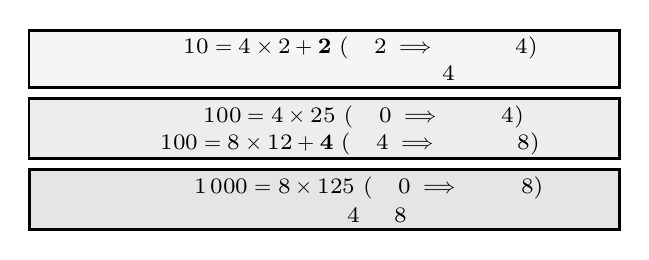
\begin{tikzpicture}[x=1cm, y=1cm, every node/.style={font=\footnotesize, text=black}]
  \draw[black, line width=0.95pt, fill=gray!8] (0,1.80) rectangle (7.50,2.52);
  \node at (3.75,2.30) {\textbf{កញ្ចប់ ១០៖} $10 = 4\times 2 + \mathbf{2}$ (សល់ $2 \implies$ មិនដាច់នឹង $4$)};
  \node at (3.75,1.98) {មើលតែរាយចុង ១ ខ្ទង់ \textbf{មិនគ្រប់} សម្រាប់តួចែក $4$ ទេ};

  \draw[black, line width=0.95pt, fill=gray!14] (0,0.90) rectangle (7.50,1.66);
  \node at (3.75,1.42) {\textbf{កញ្ចប់ ១០០៖} $100 = 4\times 25$ (សល់ $0 \implies$ ដាច់នឹង $4$)};
  \node at (3.75,1.08) {ប៉ុន្តែ $100 = 8\times 12 + \mathbf{4}$ (សល់ $4 \implies$ មិនដាច់នឹង $8$)};

  \draw[black, line width=1.05pt, fill=gray!20] (0,0) rectangle (7.50,0.76);
  \node at (3.75,0.52) {\textbf{កញ្ចប់ ១\,០០០៖} $1\,000 = 8\times 125$ (សល់ $0 \implies$ ដាច់នឹង $8$)};
  \node at (3.75,0.18) {ខ្ទង់ពាន់ឡើងលើចែកដាច់នឹង $4$ និង $8$ ជានិច្ច};
\end{tikzpicture}}

% ២. E1 Engage៖ ប្រអប់សន្ទនា Concept Cartoon (សុខា vs ដារី) តម្រៀបពីលើចុះក្រោម
\newcommand{\figEngageConceptCartoon}{%
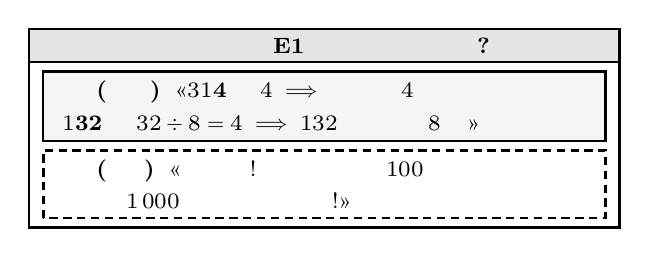
\begin{tikzpicture}[x=1cm, y=1cm, every node/.style={font=\footnotesize, text=black}]
  \fill[gray!20] (0,2.10) rectangle (7.50,2.52);
  \draw[black, line width=1.0pt] (0,0) rectangle (7.50,2.52);
  \draw[black, line width=0.7pt] (0,2.10) -- (7.50,2.10);
  \node at (3.75,2.31) {\textbf{បេសកកម្មគំនូរជជែក \en{E1} ៖ តើសុខា ឬដារី ត្រឹមត្រូវ?}};

  \draw[black, line width=0.85pt, fill=gray!8] (0.18,1.10) rectangle (7.32,1.98);
  \node[anchor=west] at (0.30,1.72) {\textbf{សុខា (អន្ទាក់)៖} «$31\mathbf{4}$ ចុង $4 \implies$ ចែកដាច់នឹង $4$ ហើយ};
  \node[anchor=west] at (0.30,1.32) {$1\mathbf{32}$ មាន $32\div 8 = 4 \implies 132$ ក៏ចែកដាច់នឹង $8$ ដែរ»};

  \draw[black, line width=0.95pt, densely dashed, fill=white] (0.18,0.12) rectangle (7.32,0.98);
  \node[anchor=west] at (0.30,0.72) {\textbf{ដារី (សង្ស័យ)៖} «មិនប្រាកដទេ! ត្រូវពិនិត្យកញ្ចប់ $100$};
  \node[anchor=west] at (0.30,0.34) {និងប្រអប់ $1\,000$ ជាមុន មុននឹងសម្រេចចិត្ត!»};
\end{tikzpicture}}

% ៣. E2 Explore ស្ថានីយទី១៖ គំនូរបំបែកកញ្ចប់ ១០០ សម្រាប់តួចែក ៤ (១២៤ ទល់នឹង ៣១៤)
\newcommand{\figExploreBundleFour}{%
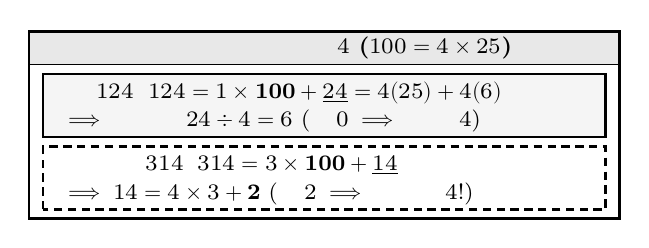
\begin{tikzpicture}[x=1cm, y=1cm, every node/.style={font=\footnotesize, text=black}]
  \fill[gray!18] (0,1.96) rectangle (7.50,2.38);
  \draw[black, line width=1.0pt] (0,0) rectangle (7.50,2.38);
  \draw[black, line width=0.7pt] (0,1.96) -- (7.50,1.96);
  \node at (3.75,2.17) {\textbf{ពិសោធន៍កញ្ចប់ ១០០ សម្រាប់តួចែក $4$ ($100 = 4\times 25$)}};

  \draw[black, line width=0.85pt, fill=gray!8] (0.18,1.04) rectangle (7.32,1.84);
  \node[anchor=west] at (0.30,1.60) {\textbf{ករណី $124$៖} $124 = 1\times \mathbf{100} + \underline{24} = 4(25) + 4(6)$};
  \node[anchor=west] at (0.30,1.24) {$\implies$ ២ ខ្ទង់ចុង $24 \div 4 = 6$ (សល់ $0 \implies$ ដាច់នឹង $4$)};

  \draw[black, line width=0.85pt, densely dashed, fill=white] (0.18,0.12) rectangle (7.32,0.92);
  \node[anchor=west] at (0.30,0.68) {\textbf{ឧទាហរណ៍ផ្ទុយ $314$៖} $314 = 3\times \mathbf{100} + \underline{14}$};
  \node[anchor=west] at (0.30,0.32) {$\implies 14 = 4\times 3 + \mathbf{2}$ (សល់ $2 \implies$ មិនដាច់នឹង $4$!)};
\end{tikzpicture}}

% ៤. E2 Explore ស្ថានីយទី២៖ គំនូរបំបែកកញ្ចប់ ១០០០ សម្រាប់តួចែក ៨ (៣១២៨ ទល់នឹង ១៣២)
\newcommand{\figExploreBundleEight}{%
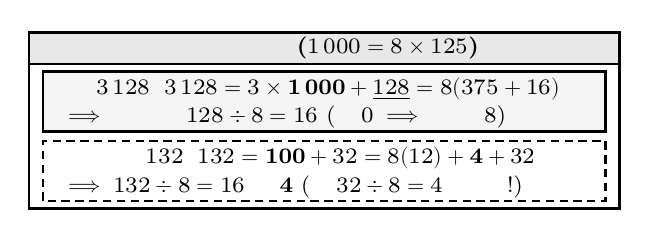
\begin{tikzpicture}[x=1cm, y=1cm, every node/.style={font=\footnotesize, text=black}]
  \fill[gray!18] (0,1.84) rectangle (7.50,2.24);
  \draw[black, line width=1.0pt] (0,0) rectangle (7.50,2.24);
  \draw[black, line width=0.7pt] (0,1.84) -- (7.50,1.84);
  \node at (3.75,2.04) {\textbf{ពិសោធន៍ប្រអប់ ១\,០០០ ($1\,000 = 8\times 125$)}};

  \draw[black, line width=0.85pt, fill=gray!8] (0.18,0.98) rectangle (7.32,1.74);
  \node[anchor=west] at (0.30,1.52) {\textbf{ករណី $3\,128$៖} $3\,128 = 3\times \mathbf{1\,000} + \underline{128} = 8(375+16)$};
  \node[anchor=west] at (0.30,1.16) {$\implies$ ៣ ខ្ទង់ចុង $128 \div 8 = 16$ (សល់ $0 \implies$ ដាច់នឹង $8$)};

  \draw[black, line width=0.85pt, densely dashed, fill=white] (0.18,0.10) rectangle (7.32,0.86);
  \node[anchor=west] at (0.30,0.64) {\textbf{ឧទាហរណ៍ផ្ទុយ $132$៖} $132 = \mathbf{100} + 32 = 8(12)+\mathbf{4}+32$};
  \node[anchor=west] at (0.30,0.28) {$\implies 132 \div 8 = 16$ សល់ $\mathbf{4}$ (ទោះ $32\div 8=4$ ក៏មិនដាច់!)};
\end{tikzpicture}}

% ៥. E3 Explain៖ ដ្យាក្រាមរួមបញ្ឈរទំនាក់ទំនង ចែកដាច់នឹង ៨ => ចែកដាច់នឹង ៤
\newcommand{\figExplainHierarchy}{%
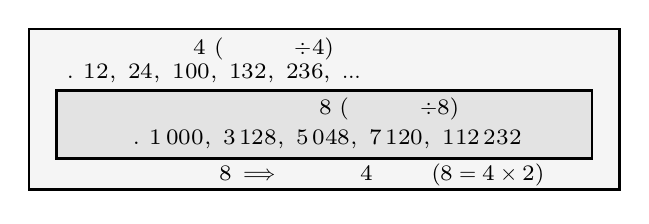
\begin{tikzpicture}[x=1cm, y=1cm, every node/.style={font=\footnotesize, text=black}]
  \draw[black, line width=0.95pt, fill=gray!8] (0,0) rectangle (7.50,2.04);
  \node[anchor=west] at (0.28,1.78) {\textbf{សំណុំចំនួនចែកដាច់នឹង $4$} (២ ខ្ទង់ចុង $\div 4$)};
  \node[anchor=west] at (0.28,1.48) {ឧ. $12,\ 24,\ 100,\ 132,\ 236,\ \dots$};

  \draw[black, line width=1.05pt, fill=gray!22] (0.35,0.40) rectangle (7.15,1.26);
  \node at (3.75,1.02) {\textbf{សំណុំរង៖ ចែកដាច់នឹង $8$} (៣ ខ្ទង់ចុង $\div 8$)};
  \node at (3.75,0.64) {ឧ. $1\,000,\ 3\,128,\ 5\,048,\ 7\,120,\ 112\,232$};

  \node at (3.75,0.18) {\textbf{វិបាក៖} ចែកដាច់នឹង $8 \implies$ ចែកដាច់នឹង $4$ ជានិច្ច ($8 = 4\times 2$)};
\end{tikzpicture}}

% ៦. E4 Elaborate៖ ដ្យាក្រាមវិភាគខ្ទង់លេខ 112 23□ (ពីរខ្ទង់ចុង vs បីខ្ទង់ចុង)
\newcommand{\figElaborateCheckBox}{%
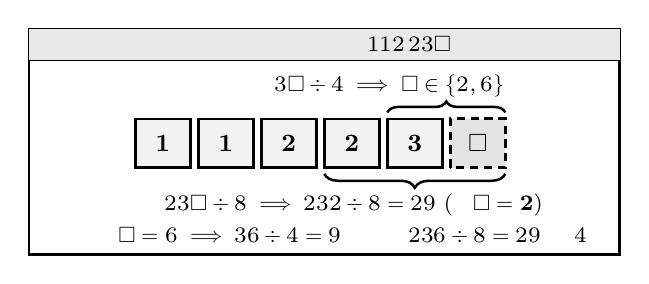
\begin{tikzpicture}[x=1cm, y=1cm, every node/.style={font=\footnotesize, text=black}]
  \draw[black, line width=0.95pt, fill=white] (0,0) rectangle (7.50,2.86);
  \fill[gray!18] (0,2.46) rectangle (7.50,2.86);
  \draw[black, line width=0.65pt] (0,2.46) -- (7.50,2.46);
  \node at (3.75,2.66) {\textbf{ផ្ទៀងលក្ខខណ្ឌ ២ ជាន់លើលេខ $112\,23\square$}};

  \foreach \i/\d in {0/1, 1/1, 2/2, 3/2, 4/3} {
    \draw[black, line width=0.9pt, fill=gray!10] (1.35+\i*0.80,1.10) rectangle (2.05+\i*0.80,1.72);
    \node[font=\small] at (1.70+\i*0.80,1.41) {\textbf{\d}};
  }
  \draw[black, line width=1.2pt, densely dashed, fill=gray!22] (5.35,1.10) rectangle (6.05,1.72);
  \node[font=\small] at (5.70,1.41) {\textbf{$\square$}};

  \draw[black, line width=0.9pt, decorate, decoration={brace, amplitude=4pt}] (4.55,1.80) -- (6.05,1.80);
  \node at (3.75,2.14) {ជំហាន ១៖ ២ ខ្ទង់ចុង $3\square \div 4 \implies \square \in \{2, 6\}$};

  \draw[black, line width=0.9pt, decorate, decoration={brace, amplitude=5pt, mirror}] (3.75,1.02) -- (6.05,1.02);
  \node at (3.75,0.62) {ជំហាន ២៖ $23\square \div 8 \implies 232\div 8 = 29$ (យក $\square = \mathbf{2}$)};

  \node at (3.75,0.24) {អន្ទាក់៖ $\square = 6 \implies 36\div 4 = 9$ ត្រូវ តែ $236\div 8 = 29$ សល់ $4$};
\end{tikzpicture}}

% ៧. E5 Exit Ticket៖ ដ្យាក្រាមវិភាគសំបុត្រចេញ 527□ (កាត់បន្ថយអន្ទាក់ 6)
\newcommand{\figExitDiagCard}{%
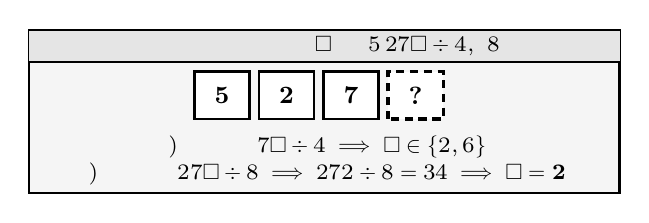
\begin{tikzpicture}[x=1cm, y=1cm, every node/.style={font=\footnotesize, text=black}]
  \draw[black, line width=0.95pt, fill=gray!8] (0,0) rectangle (7.50,2.06);
  \fill[gray!20] (0,1.66) rectangle (7.50,2.06);
  \draw[black, line width=0.65pt] (0,1.66) -- (7.50,1.66);
  \node at (3.75,1.86) {\textbf{សំបុត្រចេញ ៩០ វិនាទី៖ រក $\square$ ឱ្យ $5\,27\square \div 4,\ 8$}};

  \foreach \i/\d in {0/5, 1/2, 2/7} {
    \draw[black, line width=0.9pt, fill=white] (2.10+\i*0.82,0.94) rectangle (2.80+\i*0.82,1.54);
    \node[font=\small] at (2.45+\i*0.82,1.24) {\textbf{\d}};
  }
  \draw[black, line width=1.15pt, densely dashed, fill=white] (4.56,0.94) rectangle (5.26,1.54);
  \node[font=\small] at (4.91,1.24) {\textbf{?}};

  \node at (3.75,0.58) {១) ២ ខ្ទង់ចុង $7\square \div 4 \implies \square \in \{2, 6\}$};
  \node at (3.75,0.24) {២) ៣ ខ្ទង់ចុង $27\square \div 8 \implies 272\div 8 = 34 \implies \square = \mathbf{2}$};
\end{tikzpicture}}

% ============================================================================
% ចាប់ផ្ដើមឯកសារ (Document Body)
% ============================================================================
\begin{document}
\fontsize{10pt}{15.2pt}\selectfont

% -------------------- ក្បាលរដ្ឋបាល --------------------
{\centering
  {\muol\fontsize{11pt}{16pt}\selectfont ព្រះរាជាណាចក្រកម្ពុជា\par}
  {\muol\fontsize{10.5pt}{15pt}\selectfont ជាតិ សាសនា ព្រះមហាក្សត្រ\par}
  \vspace{-3pt}{\khmflourish\par}
}

\vspace{-22pt}
{\muol\fontsize{9.6pt}{13.2pt}\selectfont
មន្ទីរអប់រំ យុវជន និងកីឡា ខេត្តកំពង់ធំ\\
ការិយាល័យអប់រំ យុវជន និងកីឡា ស្រុកកំពង់ស្វាយ\\
អនុវិទ្យាល័យព្រះក្រសាំង\par}

\vspace{2pt}
{\centering{\muol\fontsize{11pt}{16pt}\selectfont កិច្ចតែងការបង្រៀន\par}}
\vspace{2pt}

% -------------------- ព័ត៌មានទូទៅ --------------------
{\renewcommand{\arraystretch}{1.04}
\hspace*{3.3cm}%
\begin{tabular}{@{}l@{\hspace{0.35cm}}p{2.95cm}@{\hspace{0.15cm}}c@{\hspace{0.25cm}}l@{}}
  - & មុខវិជ្ជា & : & គណិតវិទ្យា ថ្នាក់ទី៧ (ពីជគណិត) \\
  - & ចំណងជើងមេរៀន & : & មេរៀនទី២៖ តួចែកនិងពហុគុណ \\
  - & ចំណងជើងរង & : & ១.១ គ. ភាពចែកដាច់នឹង $4$ និង $8$ (ទំ.១៧) \\
  - & រយៈពេល & : & ១ ម៉ោងសិក្សា (៥០ នាទី) \\
  - & បង្រៀនដោយ & : & ហុក ប៊ុនថែន \\
  - & កាលបរិច្ឆេទ & : & ថ្ងៃសុក្រ ទី១៣ ខែវិច្ឆិកា ឆ្នាំ២០២៦ \\
\end{tabular}\par}

\vspace{5pt}

% -------------------- I. វត្ថុបំណង --------------------
{\muol\fontsize{10pt}{15pt}\selectfont \enbf{I.} វត្ថុបំណង\par}
\vspace{1.5pt}
{\renewcommand{\arraystretch}{1.10}
\begin{tabular}{@{}p{0.48cm}@{\hspace{0.22cm}}p{2.45cm}@{\hspace{0.15cm}}c@{\hspace{0.25cm}}L{14.70cm}@{}}
  \hfill\wcirc & វិជ្ជាសម្បទា & : & សិស្សប្រាប់បានពីលក្ខណៈចែកដាច់នៃចំនួនគត់នឹង $4$ (មើលលេខខាងចុងពីរខ្ទង់) និងនឹង $8$ (មើលលេខខាងចុងបីខ្ទង់) ព្រមទាំងពន្យល់ហេតុផលតាមរចនាសម្ព័ន្ធគោលដប់ ($100 = 4\times 25$, $1\,000 = 8\times 125$) បានត្រឹមត្រូវ ។ \\
  \hfill\wcirc & បំណិនសម្បទា & : & សិស្សកំណត់ភាពចែកដាច់នៃចំនួនធំដោយមិនបាច់ធ្វើវិធីចែកទាំងស្រុង និងបំពេញលេខក្នុងប្រអប់ $\square$ ឱ្យចំនួនចែកដាច់នឹង $4$ ផង និង $8$ ផង (លំហាត់គំរូ និងប្រតិបត្តិទំ.១៧) បានត្រឹមត្រូវគ្រប់ជំហាន ។ \\
  \hfill\wcirc & ចរិយាសម្បទា & : & សិស្សមានភាពម៉ត់ចត់មិនច្រឡំមើលតែខ្ទង់រាយ មិនភ្លេចលេខ $0$ ក្នុងប្រអប់ និងផ្ទៀងផ្ទាត់ហេតុផលលេខវិទ្យាជាក្រុមដោយការទទួលខុសត្រូវ ។ \\
\end{tabular}\par}

\vspace{5pt}

% -------------------- II. សម្ភារៈឧបទេស --------------------
{\muol\fontsize{10pt}{15pt}\selectfont \enbf{II.} សម្ភារៈឧបទេស\par}
\vspace{1.5pt}
\begin{clist}
  \item សៀវភៅសិក្សាគោលគណិតវិទ្យា ថ្នាក់ទី៧ (ទំ.១៧ និងទំ.២៤) ក្ដារខៀន ៣ ផ្នែក ដីស/ហ្វឺត និងបន្ទាត់
  \item សន្លឹកកិច្ចការសិស្ស ស-ខ្មៅ (\en{Worksheet\_DIV21c} ទំព័រ ១--៣) ព្រីនចែកសិស្សម្នាក់ ១ កញ្ចប់ (គ្មានស្លាយ \en{LCD})
\end{clist}

\vspace{5pt}

% -------------------- III. វិធីសាស្រ្តបង្រៀន --------------------
{\muol\fontsize{10pt}{15pt}\selectfont \enbf{III.} វិធីសាស្រ្តបង្រៀន\par}
\vspace{1.5pt}
{\renewcommand{\arraystretch}{1.08}
\begin{tabular}{@{}p{0.48cm}@{\hspace{0.22cm}}p{2.45cm}@{\hspace{0.15cm}}c@{\hspace{0.25cm}}L{14.70cm}@{}}
  \hfill$\bullet$ & គោលវិធី & : & សិស្សមជ្ឈមណ្ឌល (សន្លឹកកិច្ចការពិសោធន៍ស-ខ្មៅ ៣ ទំព័រ និងការសហការគិតជាដៃគូ--ក្រុម ៣ នាក់) \\
  \hfill$\bullet$ & យុទ្ធវិធីបង្រៀន & : & គំរូស្ថាបនានិយម \en{5Es} រួមផ្សំគំនូរជជែកអន្ទាក់ (\en{Concept Cartoons}) ការរកឃើញតាមតម្លៃខ្ទង់ ($100,\ 1\,000$) និងលំដាប់គំរូត្រឹមត្រូវមុន--អន្ទាក់ក្រោយ (\en{EFWE + CIWE + EIA}) \\
\end{tabular}\par}

\vspace{4pt}

% -------------------- IV. ដំណើរការបង្រៀន --------------------
{\muol\fontsize{10pt}{15pt}\selectfont \enbf{IV.} ដំណើរការបង្រៀន\par}

{\renewcommand{\arraystretch}{1.04}
\begin{longtable}{|L{5.50cm}|L{7.90cm}|L{4.80cm}|}
\hline
\multicolumn{1}{|c|}{\cellcolor{headgray}\muol សកម្មភាពគ្រូ} &
\multicolumn{1}{c|}{\cellcolor{headgray}\muol ខ្លឹមសារមេរៀន} &
\multicolumn{1}{c|}{\cellcolor{headgray}\muol សកម្មភាពសិស្ស} \\
\hline
\endfirsthead

\hline
\multicolumn{1}{|c|}{\cellcolor{headgray}\muol សកម្មភាពគ្រូ} &
\multicolumn{1}{c|}{\cellcolor{headgray}\muol ខ្លឹមសារមេរៀន} &
\multicolumn{1}{c|}{\cellcolor{headgray}\muol សកម្មភាពសិស្ស} \\
\hline
\endhead

\hline
\endfoot

\hline
\endlastfoot

% ==================== ជំហានទី១ (2min) ====================
\stepheader{ជំហានទី១ \enbf{(}រដ្ឋបាលថ្នាក់\enbf{)}}
\timenote{(2min)}
\begin{tlist}
  \item ពិនិត្យអវត្តមាន សណ្ដាប់ធ្នាប់ និងអនាម័យថ្នាក់រៀន
  \item ចែក \textbf{សន្លឹកកិច្ចការ \en{DIV21c} (ទំព័រ ១--៣)} ជូនសិស្សម្នាក់ ១ កញ្ចប់ដាក់ផ្កាប់លើតុ
\end{tlist}
&
\begin{clist}
  \item រដ្ឋបាលថ្នាក់ សណ្ដាប់ធ្នាប់ និងត្រៀមសៀវភៅសិក្សាគោលថ្នាក់ទី៧ (ទំ.១៧) ។
  \item សន្លឹកកិច្ចការស-ខ្មៅ \en{DIV21c} (ទំព័រ ១--៣) ។
\end{clist}
&
\begin{slist}
  \item ប្រធានថ្នាក់រាយការណ៍វត្តមានសិស្ស
  \item ទទួលសន្លឹកកិច្ចការផ្កាប់ទុកលើតុ និងរៀបក្រុម ៣ នាក់
\end{slist} \\
\hline

% ==================== ជំហានទី២ (9min: <=3 + 3 + E1 3) ====================
\stepheader{ជំហានទី២ \enbf{(}ពិនិត្យចំណេះដឹងមុន \enbf{+} ទំនាក់ទំនងមេរៀនថ្មី\enbf{)}}
\ditem \textbf{ពិនិត្យកិច្ចការផ្ទះ ($\le 3\unit{min}$)} \timenote{កែលំហាត់ម៉ោងមុន}
\begin{tlist}
  \item ហៅសិស្សម្នាក់ឡើងសរសេរដំណោះស្រាយលេខ ១ ទំ.២៤ លើក្ដារខៀនឆ្វេង
\end{tlist}
&
{\redsub{កំណែលំហាត់ទំ.២៤ (កិច្ចការផ្ទះម៉ោងមុន \en{DIV21})}}\par
\textbf{លេខ ១ (បញ្ជាក់ភាពចែកដាច់ដោយមិនចែក)៖}\par
$\displaystyle\begin{aligned}
  &\text{ក. } 78 + 120 = 198 &&(\text{រាយ } 8 \text{ គូ} \implies \div 2) \\
  &\text{ខ. } 4\,140 - 720 = 3\,420 &&(\text{បូកខ្ទង់ } 9 \implies \div 3) \\
  &\text{គ. } 165 + 270 = 435 &&(\text{រាយ } 5 \implies \div 5) \\
  &\text{ឃ. } 5\,130 - 342 = 4\,788 &&(\text{បូកខ្ទង់ } 27 \implies \div 9)
\end{aligned}$
&
\begin{slist}
  \item ឡើងកែលំហាត់ទំ.២៤ លេខ ១ លើក្ដារខៀន
  \item ផ្ទៀងចម្លើយលេខ ១ ក្នុងសៀវភៅកិច្ចការផ្ទះ
\end{slist} \\[3pt]

\begin{tlist}
  \item ហៅសិស្សម្នាក់ទៀតសរសេរលេខ ២ ($734\square 0$) និងផ្ទៀងផ្ទាត់ផ្លូវការរួមគ្នា
\end{tlist}
&
\textbf{លេខ ២ ($734\square 0$)៖}\par
$\displaystyle\begin{aligned}
  &\text{ក. ដាច់នឹង } 2, 5\text{៖ } \text{រាយ } 0 \text{ ស្រាប់} \implies \square \in \{0,1,\dots,9\} \\
  &\text{ខ. ដាច់នឹង } 3, 9\text{៖ } 14 + \square = 18 \implies \square = \mathbf{4}\ (73\,440)
\end{aligned}$
&
\begin{slist}
  \item ឡើងកែលំហាត់ទំ.២៤ លេខ ២ លើក្ដារខៀន
\end{slist} \\[3pt]

\ditem \textbf{រំលឹកមេរៀនទាក់ទង (3min)}
\begin{tlist}
  \item សួររំលឹកហេតុផលនៃក្បួន $2, 5$ ($10 = 2\times 5$) និង $3, 9$ ($10 = 9+1$)
  \item ឱ្យសិស្សសាកចែក $10$, $100$ និង $1\,000$ នឹង $4$ ហើយនិង $8$
\end{tlist}
&
{\redsub{រំលឹកតម្លៃខ្ទង់គោលដប់ក្រោមតួចែក $4$ និង $8$}} \par
$\displaystyle\begin{aligned}
  10 &= 4 \times 2 + \mathbf{2} &&(\text{មិនចែកដាច់នឹង } 4) \\
  100 &= 4 \times 25 + \mathbf{0} &&(\text{ចែកដាច់នឹង } 4) \\
  100 &= 8 \times 12 + \mathbf{4} &&(\text{មិនចែកដាច់នឹង } 8) \\
  1\,000 &= 8 \times 125 + \mathbf{0} &&(\text{ចែកដាច់នឹង } 8)
\end{aligned}$
&
\begin{slist}
  \item ឆ្លើយលទ្ធផលចែក $10, 100, 1\,000$ នឹង $4$ និង $8$
  \item កត់សម្គាល់ $100\div 4$ និង $1\,000\div 8$
\end{slist} \\[3pt]

&
\cfig{\figPrereqFourEight}
& \\[3pt]

\fiveE{E1 - Engage (3min)} \timenote{(កុំទាន់ប្រាប់ចម្លើយ)}
\begin{tlist}
  \item ឱ្យសិស្សបើក \textbf{សន្លឹកកិច្ចការទំព័រ ១} អាន \textbf{គំនូរជជែកបេសកកម្ម \en{E1}} រវាង \textbf{សុខា} និង \textbf{ដារី}
  \item សួរបំផុសថាតើសុខា ឬដារី និយាយត្រឹមត្រូវ ហើយហេតុអ្វីយើងមិនអាចមើលតែលេខរាយ $4$ ដូចតួចែក $2$ បាន
\end{tlist}
&
{\redsub{បេសកកម្មគំនូរជជែក \en{E1} ៖ ពិនិត្យសំបុត្រលេខ $314$ និង $132$}}
\begin{clist}
  \item \textbf{សុខាអះអាង៖} «$31\mathbf{4}$ ចុង $4 \implies$ ចែកដាច់នឹង $4$ ហើយ $1\mathbf{32}$ មាន $32\div 8=4 \implies$ ចែកដាច់នឹង $8$ ។»
  \item \textbf{ដារីតប៖} «កុំប្រញាប់ជឿ! $10$ មិនដាច់នឹង $4$ ទេ ហើយ $100$ ក៏មិនដាច់នឹង $8$ ដែរ ។»
\end{clist}
&
\begin{slist}
  \item អានប្រអប់សន្ទនា \en{E1} លើសន្លឹកកិច្ចការទំព័រ ១
  \item ពិភាក្សាជាដៃគូ ៤៥ វិនាទី និងគូសធីកទស្សន៍ទាយដំបូង
\end{slist} \\[3pt]

&
\cfig{\figEngageConceptCartoon}
& \\
\hline

% ==================== ជំហានទី៣ (17min: E2 11m + E3 6m) ====================
\stepheader{ជំហានទី៣ \enbf{(}ខ្លឹមសារមេរៀនថ្មី\enbf{)}}
\fiveE{E2 - Explore (11min)}
\begin{tlist}
  \item សរសេរចំណងជើងរង \textbf{គ. ភាពចែកដាច់នឹង $4$ និង $8$ (ទំ.១៧)}
  \item \textbf{ស្ថានីយទី១ (5.5min)៖} ណែនាំសិស្សបំពេញ \textbf{តារាងបំបែកកញ្ចប់ ១០០} លើសន្លឹកកិច្ចការ (ឧទាហរណ៍ ១ ទំ.១៧ និងឧទាហរណ៍ផ្ទុយ $114,\ 314$)
\end{tlist}
&
{\redsub{គ. ភាពចែកដាច់នឹង $4$ និង $8$ (សៀវភៅគោល ទំ.១៧)}} \par
\textbf{១. ពិសោធន៍កញ្ចប់ ១០០ រកក្បួនតួចែក $4$ (ឧទាហរណ៍ ១ ទំ.១៧)៖}\par
$\displaystyle\begin{aligned}
  124 &= 1\times 100 + 24 &&(24\div 4 = 6,\ \text{ដាច់}) \\
  832 &= 8\times 100 + 32 &&(32\div 4 = 8,\ \text{ដាច់}) \\
  1\,000 &= 10\times 100 + 00 &&(00\div 4 = 0,\ \text{ដាច់}) \\
  314 &= 3\times 100 + 14 &&(14\div 4 = 3 \text{ សល់ } 2)
\end{aligned}$
&
\begin{slist}
  \item កត់ចំណងជើងរង និងបំពេញតារាងស្ថានីយទី១
  \item បំបែក $124,\ 832,\ 1\,000$ ធៀបនឹង $114,\ 314$ រួចទាញសន្និដ្ឋានពីរខ្ទង់ចុង
\end{slist} \\[3pt]

&
\cfig{\figExploreBundleFour}
& \\[3pt]

\begin{tlist}
  \item \textbf{ស្ថានីយទី២ (5.5min)៖} ឱ្យសិស្សបន្តទៅ \textbf{សន្លឹកកិច្ចការទំព័រ ២} បំពេញ \textbf{តារាងបំបែកប្រអប់ ១\,០០០} (ឧទាហរណ៍ ២ ទំ.១៧ និងឧទាហរណ៍ផ្ទុយ $132$)
\end{tlist}
&
\textbf{២. ពិសោធន៍ប្រអប់ ១\,០០០ រកក្បួនតួចែក $8$ (ឧទាហរណ៍ ២ ទំ.១៧)៖}\par
$\displaystyle\begin{aligned}
  3\,128 &= 3\times 1\,000 + 128 &&(128\div 8 = 16,\ \text{ដាច់}) \\
  5\,048 &= 5\times 1\,000 + 048 &&(048\div 8 = 6,\ \text{ដាច់}) \\
  7\,120 &= 7\times 1\,000 + 120 &&(120\div 8 = 15,\ \text{ដាច់}) \\
  132 &= 1\times 100 + 32 &&(132 = 8\times 16 + 4)
\end{aligned}$
&
\begin{slist}
  \item បើកសន្លឹកកិច្ចការទំព័រ ២ បំពេញតារាងស្ថានីយទី២
  \item សង្កេត $048$ មាន $0$ នៅខ្ទង់រយ និង $132$ មិនដាច់នឹង $8$
\end{slist} \\[3pt]

&
\cfig{\figExploreBundleEight}
& \\[3pt]

\fiveE{E3 - Explain (6min)}
\begin{tlist}
  \item ឱ្យតំណាងក្រុមឡើងរាយការណ៍លទ្ធផលស្ថានីយ ១--២ រួចសង្ខេបប្រអប់ \textbf{«ជាទូទៅ»} ដូចសៀវភៅសិក្សាគោល
\end{tlist}
&
\noindent\fbox{\parbox{7.45cm}{\raggedright
\textbf{ជាទូទៅ}\par
\begin{sublist}
  \item មួយចំនួនចែកដាច់នឹង 4 កាលណាវាមានលេខខាងចុងពីរខ្ទង់ចែកដាច់នឹង 4
  \item មួយចំនួនចែកដាច់នឹង 8 កាលណាវាមានលេខខាងចុងបីខ្ទង់ចែកដាច់នឹង 8 ។
\end{sublist}
}}
&
\begin{slist}
  \item រាយការណ៍សន្និដ្ឋានពីលទ្ធផលពិសោធន៍
  \item កត់ប្រអប់ «ជាទូទៅ» លើសន្លឹកកិច្ចការ
\end{slist} \\[3pt]

\begin{tlist}
  \item ពន្យល់ទំនាក់ទំនង $\div 8 \implies \div 4$ និង \textbf{ធនាគារហេតុផល \cnum{1}--\cnum{4}}
\end{tlist}
&
\textbf{ធនាគារហេតុផល (\en{Warrant Bank})៖}
\begin{clist}
  \item[\cnum{1}] \textbf{ដាច់នឹង $4$៖} លេខខាងចុងពីរខ្ទង់ចែកដាច់នឹង $4$ (រួមទាំង $00$) ។
  \item[\cnum{2}] \textbf{ដាច់នឹង $8$៖} លេខខាងចុងបីខ្ទង់ចែកដាច់នឹង $8$ (រួមទាំង $000$ ឬ $048$) ។
  \item[\cnum{3}] \textbf{វិបាក $8 \implies 4$៖} ចែកដាច់នឹង $8 \implies$ ចែកដាច់នឹង $4$ ជានិច្ច (ច្រាសមកវិញមិនពិត ឧ. $132$) ។
  \item[\cnum{4}] \textbf{លក្ខខណ្ឌរួមគ្នា៖} ត្រូវចែកដាច់នឹង $4$ ផង និង $8$ ផង គឺពិនិត្យលក្ខខណ្ឌ \cnum{1} រួចផ្ទៀងលក្ខខណ្ឌ \cnum{2} ។
\end{clist}
&
\begin{slist}
  \item ផ្ទៀងលេខកូដហេតុផល \cnum{1}--\cnum{4} លើសន្លឹកកិច្ចការ
\end{slist} \\[3pt]

&
\cfig{\figExplainHierarchy}
& \\
\hline

% ==================== ជំហានទី៤ (20min: E4 10m + E5 10m) ====================
\stepheader{ជំហានទី៤ \enbf{(}ពង្រីកចំណេះដឹង\enbf{)}}
\fiveE{E4 - Elaborate (10min)}
\begin{tlist}
  \item ណែនាំសិស្សបើក \textbf{សន្លឹកកិច្ចការទំព័រ ៣ (ផ្នែក ឃ)}
\end{tlist}
&
{\muol លំហាត់គំរូ ១} \textbf{(សៀវភៅគោល ទំ.១៧)៖} គេឱ្យចំនួនមានលេខ $6$ ខ្ទង់ $112\,23\square$ ។ ចូរបំពេញលេខក្នុងប្រអប់ដើម្បីឱ្យចំនួននោះចែកដាច់នឹង $4$ ផង និង $8$ ផង ។
&
\begin{slist}
  \item អានប្រធានលំហាត់គំរូ ១ លើសន្លឹកកិច្ចការទំព័រ ៣
\end{slist} \\[3pt]

\begin{tlist}
  \item បង្ហាញជំហានទី ១ នៃ \textbf{លំហាត់គំរូ ១} ជាគំរូត្រឹមត្រូវមុន (\en{Correct-First EFWE})
\end{tlist}
&
\textbf{ជំហាន ១ (ព្រោះតួចែក $4$ គូ នោះ $\square \in \{0,2,4,6,8\}$; ពិនិត្យ $3\square \div 4$ តាម \cnum{1})៖}\par
$\displaystyle\begin{aligned}
  30 \div 4 &= 7\ (\text{សល់ } 2) \;\; & 32 \div 4 &= 8\ (\text{សល់ } 0\text{ — យក}) \\
  34 \div 4 &= 8\ (\text{សល់ } 2) \;\; & 36 \div 4 &= 9\ (\text{សល់ } 0\text{ — យក}) \\
  38 \div 4 &= 9\ (\text{សល់ } 2) \;\; &\implies \square &\in \{2,\ 6\}
\end{aligned}$
&
\begin{slist}
  \item តាមដានជំហានទី ១ លើក្ដារខៀន និងផ្ទៀង $\square \in \{2,\ 6\}$
\end{slist} \\[3pt]

\begin{tlist}
  \item បន្តបង្ហាញជំហានទី ២ ផ្ទៀង ៣ ខ្ទង់ចុងនឹង $8$
\end{tlist}
&
\textbf{ជំហាន ២ (ពិនិត្យ ៣ ខ្ទង់ចុង $23\square \div 8$ តាម \cnum{2})៖}\par
$\displaystyle\begin{aligned}
  &\square = 2 \text{៖ } 232 \div 8 = 29\ (\text{សំណល់ } 0 \implies \text{ដាច់នឹង } 8) \\
  &\square = 6 \text{៖ } 236 \div 8 = 29\ (\text{សំណល់ } 4 \ne 0 \implies \text{មិនដាច់!})
\end{aligned}$
&
\begin{slist}
  \item ផ្ទៀង $232\div 8$ និង $236\div 8$ លើសន្លឹកកិច្ចការ
\end{slist} \\[3pt]

\begin{tlist}
  \item សរុបចម្លើយលំហាត់គំរូ ១
\end{tlist}
&
\textbf{សន្និដ្ឋាន៖} $\graybox{$\square = 2$},\ \graybox{$112\,232$}$ (ដាច់នឹង $4$ និង $8$) ។
&
\begin{slist}
  \item បំពេញ $\square = 2$ លើទំព័រ ៣
\end{slist} \\[3pt]

&
\cfig{\figElaborateCheckBox}
& \\[3pt]

\begin{tlist}
  \item ឱ្យសិស្សអនុវត្តវិធីវិភាគ ២ ជំហានលើ \textbf{លំហាត់គំរូ ២ (ទំ.១៧)}
\end{tlist}
&
{\muol លំហាត់គំរូ ២} \textbf{(សៀវភៅគោល ទំ.១៧)៖} ពីឆ្នាំ $1999$ ដល់ឆ្នាំ $2010$ តើឆ្នាំណាខ្លះចែកដាច់នឹង $4$ ផង និង $8$ ផង ។
&
\begin{slist}
  \item អានប្រធានលំហាត់គំរូ ២ ជាដៃគូ
\end{slist} \\[3pt]

\begin{tlist}
  \item ពិនិត្យជំហានទី ១ សម្រាប់តួចែក $4$
\end{tlist}
&
\textbf{ជំហាន ១ (ឆ្នាំគូចែកដាច់នឹង $4$ តាម \cnum{1})៖}\par
$\displaystyle\begin{aligned}
  2000 &\to 00 \div 4 = 0 \text{ (ដាច់)} \;\; & 2002 &\to 02 \nmid 4 \\
  2004 &\to 04 \div 4 = 1 \text{ (ដាច់)} \;\; & 2006 &\to 06 \nmid 4 \\
  2008 &\to 08 \div 4 = 2 \text{ (ដាច់)} \;\; & 2010 &\to 10 \nmid 4
\end{aligned}$
&
\begin{slist}
  \item ពិនិត្យឆ្នាំគូពី $1999$ ដល់ $2010$
\end{slist} \\[3pt]

\begin{tlist}
  \item ឱ្យសិស្សផ្ទៀង ៣ ខ្ទង់ចុងនឹង $8$ ក្នុងជំហានទី ២
\end{tlist}
&
\textbf{ជំហាន ២ (ពិនិត្យ ៣ ខ្ទង់ចុងនឹង $8$ តាម \cnum{2})៖}\par
$\displaystyle\begin{aligned}
  2000 &\to 000 \div 8 = 0\ (2000 = 8\times 250 \implies \text{ដាច់}) \\
  2004 &\to 004 \div 8 = 0\ (\text{សល់ } 4 \implies \text{មិនដាច់នឹង } 8) \\
  2008 &\to 008 \div 8 = 1\ (2008 = 8\times 251 \implies \text{ដាច់})
\end{aligned}$
&
\begin{slist}
  \item រកឃើញឆ្នាំ $2008$ (និង $2000$)
\end{slist} \\[3pt]

\begin{tlist}
  \item សួរសំណួរត្រិះរិះ \textbf{\en{EIA Looking-Back} (1min)} អំពីអន្ទាក់ $\square = 6$
\end{tlist}
&
\begin{clist}
  \item \textbf{សន្និដ្ឋាន៖} ចន្លោះ $1999$--$2010$ គឺ $\graybox{$2008$}$ (និង $2000$ បើរាប់ដើមសតវត្ស $000$; សៀវភៅគោលយក $2008$) ។
  \item \textbf{\en{EIA Looking-Back}៖} $112\,236$ ចែកដាច់នឹង $4$ ($36=4\times 9$) តែមិនចែកដាច់នឹង $8$ ($236=8\times 29 + 4$) ។
\end{clist}
&
\begin{slist}
  \item ឆ្លើយសំណួរ \en{EIA} អំពីភាពខុសគ្នារវាង $232$ និង $236$
\end{slist} \\[3pt]

\fiveE{E5 - Evaluate (10min)}
\begin{tlist}
  \item \textbf{សកម្មភាពក្រុម ៣ នាក់ (4min)៖} ឱ្យសិស្សដោះស្រាយ \textbf{ប្រតិបត្តិទំ.១៧} ($734\square 0$)
\end{tlist}
&
{\muol លំហាត់ប្រតិបត្តិ} \textbf{(សៀវភៅគោល ទំ.១៧)៖} គេមានមួយចំនួនដែលមានលេខប្រាំខ្ទង់ $734\square 0$ ។ បំពេញលេខក្នុងប្រអប់ដើម្បីឱ្យចំនួននោះ៖ ក. ចែកដាច់នឹង $4$ \quad ខ. ចែកដាច់នឹង $8$ ។
&
\begin{slist}
  \item សង្កេតប្រធានលំហាត់ប្រតិបត្តិលើសន្លឹកកិច្ចការទំព័រ ៣
\end{slist} \\[3pt]

\begin{tlist}
  \item ឱ្យក្រុមសិស្សពិនិត្យ ២ ខ្ទង់ចុង $\square 0$ ក្នុងផ្នែក ក (កុំភ្លេចលេខ $0$)
\end{tlist}
&
\textbf{ក. ចែកដាច់នឹង $4$ (ពិនិត្យ ២ ខ្ទង់ចុង $\square 0$ តាម \cnum{1})៖}\par
$\displaystyle\begin{aligned}
  &\square \in \{0,2,4,6,8\}\text{៖ } 00,20,40,60,80 \text{ ដាច់នឹង } 4 \\
  &\square \in \{1,3,5,7,9\}\text{៖ } 10,30,50,70,90 \text{ សល់ } 2
\end{aligned}$
&
\begin{slist}
  \item សាកល្បងលេខ $\square = 0\dots 9$ លើ $\square 0 \div 4$
\end{slist} \\[3pt]

\begin{tlist}
  \item ឱ្យសិស្សសរុបចម្លើយទាំង ៥ នៃផ្នែក ក
\end{tlist}
&
$\displaystyle\begin{aligned}
  &\implies \graybox{$\square \in \{0,\ 2,\ 4,\ 6,\ 8\}$} \\
  &\text{ចំនួនទាំង ៥៖ } 73\,400;\ 73\,420;\ 73\,440; \\
  &\phantom{\text{ចំនួនទាំង ៥៖ }} 73\,460;\ 73\,480 \text{ ។}
\end{aligned}$
&
\begin{slist}
  \item សហការក្រុម ៣ នាក់ផ្ទៀងគ្រប់ចម្លើយទាំង ៥
\end{slist} \\[3pt]

\begin{tlist}
  \item ឱ្យក្រុមសិស្សបន្តរកផ្នែក ខ ($734\square 0$ ចែកដាច់នឹង $8$)
\end{tlist}
&
\textbf{ខ. ចែកដាច់នឹង $8$ (ពិនិត្យ $4\square 0 = 400 + \square 0$ តាម \cnum{2})៖}\par
$\displaystyle\begin{aligned}
  400 \div 8 &= 50\ (\text{យក }\mathbf{0}) \;\; & 420 \div 8 &= 52\ \text{សល់ } 4\ (\text{ទេ}) \\
  440 \div 8 &= 55\ (\text{យក }\mathbf{4}) \;\; & 460 \div 8 &= 57\ \text{សល់ } 4\ (\text{ទេ}) \\
  480 \div 8 &= 60\ (\text{យក }\mathbf{8}) \;\; & &
\end{aligned}$
&
\begin{slist}
  \item ស្វែងរក $\square \in \{0,4,8\}$ តាម ៣ ខ្ទង់ចុង
\end{slist} \\[3pt]

\begin{tlist}
  \item ផ្ទៀងផ្ទាត់ចម្លើយផ្នែក ខ និង \textbf{បិទបេសកកម្ម \en{E1}}
\end{tlist}
&
$\displaystyle \textbf{ចម្លើយ៖ } \graybox{$\square \in \{0,\ 4,\ 8\}$}$ (គឺ $73\,400;\ 73\,440;\ 73\,480$ ។)\par
\textbf{បិទបេសកកម្ម \en{E1}៖} \textbf{ដារីត្រឹមត្រូវ!} សុខាខុសទាំងពីរ ព្រោះ $314$ ($14 \nmid 4$) និង $132$ ($132 = 8\times 16 + 4 \nmid 8$) ។
&
\begin{slist}
  \item បិទបេសកកម្ម \en{E1} ដោយបញ្ជាក់ឧទាហរណ៍ផ្ទុយ $314$ និង $132$
\end{slist} \\[3pt]

\ditem \textbf{វិនិច្ឆ័យ \en{A--D} (3min)}
\begin{tlist}
  \item ឱ្យសិស្សវិនិច្ឆ័យត្រូវ/ខុសលើប្រអប់ \en{A,\ B}
\end{tlist}
&
\textbf{វិនិច្ឆ័យ \en{A--D} (\en{Correct-Incorrect Critique})៖}
\begin{clist}
  \item \textbf{A (ខុស \ding{55} — កូដ \cnum{1})៖} $314$ ចុង $4$ តែ ២ ខ្ទង់ចុង $14$ មិនចែកដាច់នឹង $4$ ។
  \item \textbf{B (ខុស \ding{55} — កូដ \cnum{2})៖} $132$ មាន $32\div 8=4$ តែ ៣ ខ្ទង់ចុង $132\div 8=16$ សល់ $4$ ។
\end{clist}
&
\begin{slist}
  \item គូសត្រូវ/ខុស \en{A,\ B} និងរាយការណ៍លេខកូដ
\end{slist} \\[3pt]

\begin{tlist}
  \item បន្តឱ្យសិស្សវិនិច្ឆ័យ \en{C,\ D} រួចលើកម្រាមដៃ (១=ត្រូវ, ២=ខុស)
\end{tlist}
&
\begin{clist}
  \item \textbf{C (ត្រូវ \ding{51} — កូដ \cnum{3})៖} ចែកដាច់នឹង $8 \implies$ ចែកដាច់នឹង $4$ ជានិច្ច ($8=4\times 2$) ។
  \item \textbf{D (ត្រូវ \ding{51} — កូដ \cnum{1},\cnum{2})៖} $73\,400$ មាន $00\div 4=0$ និង $400\div 8=50$ ។
\end{clist}
&
\begin{slist}
  \item គូស \en{C,\ D} និងលើកម្រាមដៃបង្ហាញគ្រូព្រមគ្នា
\end{slist} \\[3pt]

\ditem \textbf{សំបុត្រចេញ ៩០ វិនាទី (3min)}
\begin{tlist}
  \item ប្រមូល \textbf{សំបុត្រចេញ ៩០ វិនាទី} ($5\,27\square$) មុនបញ្ចប់ម៉ោង
\end{tlist}
&
\textbf{សំបុត្រចេញ ៩០ វិនាទី ($5\,27\square$ ចែកដាច់នឹង $4$ និង $8$)៖}\par
$\displaystyle\begin{aligned}
  &\text{១) ២ ខ្ទង់ចុង } 7\square \div 4 \implies \square \in \{2,\ 6\} \\
  &\text{២) ៣ ខ្ទង់ចុង៖ } 272 \div 8 = 34\ (\text{សល់ } 0,\ \text{យក}) \\
  &\phantom{\text{២) ៣ ខ្ទង់ចុង៖ }} 276 \div 8 = 34\ (\text{សល់ } 4,\ \text{មិនយក}) \\
  &\implies \graybox{$\square = 2$} \quad (5\,272) \text{ ។}
\end{aligned}$
&
\begin{slist}
  \item បំពេញសំបុត្រចេញ $5\,27\mathbf{2}$ ដោយឯករាជ្យក្នុង ៩០ វិនាទី
\end{slist} \\[3pt]

&
\cfig{\figExitDiagCard}
& \\
\hline

% ==================== ជំហានទី៥ (<=2min) ====================
\stepheader{ជំហានទី៥ \enbf{(}កិច្ចការផ្ទះ \enbf{+} បណ្ដាំផ្ញើ\enbf{)}}
\timenote{(កុំឱ្យលើស 2min)}
\begin{tlist}
  \item ណែនាំលំហាត់ពង្រឹង ១ លើសន្លឹកកិច្ចការទំព័រ ៣
\end{tlist}
&
{\muol កិច្ចការផ្ទះ} \textbf{(លំហាត់ពង្រឹង $4$ និង $8$)៖}
\begin{clist}
  \item \textbf{លំហាត់ ១៖} កំណត់ថាតើចំនួន $4\,216;\ 9\,132;\ 12\,500;\ 8\,408$ ចែកដាច់នឹង $4$ ឬ $8$ ឬទាំងពីរ ដោយបង្ហាញ ២ ខ្ទង់ និង ៣ ខ្ទង់ចុង ។
\end{clist}
&
\begin{slist}
  \item កត់ត្រាលំហាត់ ១ ចូលសៀវភៅកិច្ចការផ្ទះ
\end{slist} \\[3pt]

\begin{tlist}
  \item បញ្ជាក់លំហាត់ ២ (ប្រយ័ត្នចម្លើយលើសពី ១)
\end{tlist}
&
\begin{clist}
  \item \textbf{លំហាត់ ២៖} បំពេញលេខក្នុងប្រអប់នៃ $61\,3\square 6$ ដើម្បីឱ្យចែកដាច់នឹង $4$ ផង និង $8$ ផង ។
\end{clist}
&
\begin{slist}
  \item កត់ត្រាលំហាត់ ២ ចូលសៀវភៅកិច្ចការផ្ទះ
\end{slist} \\[3pt]

\begin{tlist}
  \item ផ្ដាំផ្ញើសិស្សអានមុនចំណុច ១.២ ទំ.១៨
\end{tlist}
&
\begin{clist}
  \item \textbf{បណ្ដាំផ្ញើ៖} អានមុន \textbf{១.២ លក្ខណៈចែកដាច់នៃផលបូកនិងផលដក (ទំ.១៨)} ។
\end{clist}
&
\begin{slist}
  \item ទុកសន្លឹកកិច្ចការឱ្យមានរបៀប និងជម្រាបលាគ្រូ
\end{slist} \\
\hline
\end{longtable}}

% -------------------- ហត្ថលេខា (ចន្ទគតិ + សុរិយគតិ ត្រូវគ្នា ១០០%) --------------------
\vspace{8pt}
\noindent\hfill
\begin{minipage}{9.6cm}
  \centering
  ថ្ងៃសុក្រ ៤កើត ខែកត្តិក ឆ្នាំមមី អដ្ឋស័ក ពុទ្ធសករាជ ២៥៧០\\[2pt]
  កំពង់ស្វាយ, ថ្ងៃទី១៣ ខែវិច្ឆិកា ឆ្នាំ២០២៦\\[4pt]
  {\muol\fontsize{10.5pt}{15pt}\selectfont គ្រូបង្រៀន}\\[32pt]
  \hfill{\muol\fontsize{10.5pt}{15pt}\selectfont ហុក ប៊ុនថែន}\hspace*{1.4cm}
\end{minipage}

\end{document}
